\documentclass[12pt,a4paper]{report}

\usepackage[pdftex]{graphicx}

\begin{document}


\title{Qedo Run-Time Environment - Documentation}
\author{Harald Boehme \\ Bertram Neubauer \\ Tom Ritter \\ Frank Stoinski}

\maketitle

\setcounter{page}{1} 

\tableofcontents


\chapter{Introduction}
\label{sec:Introduction}

The Qedo Run-Time.

...
\section{Installation}
\label{sec:Installation}
For the Installation of the run-time consult the Installation Guide.


\section{Contact}
\label{sec:Contact}

If you have any problem or if you have any comments do not hesitate to contact the other Qedo users by using the qedo-devel mailing list. You can reach it at qedo-devel@lists.berlios.de. You can also use the bug tracking system provided by the Qedo project. You can reach it at \verb http://www.qedo.org . this site has all relevant information about the Qedo project. In any case you can also contact the authors directly. The email addresses are listed on the Qedo web page as well.




\chapter{Architecture}
\label{sec:Architecture}
Qedo run-time has the following architecture.

 ...

\section{Component Server}
\label{sec:ComponentServer}
The component server is the actual run-time environment of a component.  

 ... 

\section{Component Container}
\label{sec:ComponentContainer}
The Component Container is a kind of an administrative entity within the component server. It offers interface to the component and the component uses interfaces of the container.

...

\section{Component Installer}
\label{sec:ComponentInstaller}
The Component Installer is used to install the binaries of the components, before that can be loaded into the component server.

...

\chapter{Usage}
\label{sec:Usage}
This section explain the options. ...

\section{Configuration File}
\label{sec:ConfigurationFile}
The Qedo run-time environment is complex software and provides a set of functionalities. Sometimes there are different ways how to provide the functionality. To allow an easy configuration of such properties at run-time (instead of compile-time) Qedo provides a configuration file. XML is used in this file, to make the integration with other tools easier. Though this file is not complex and can be edited with a normal text editor. The following will guide you through the different sections of this file.

The file is structured in sections. Each section can have nested sections or configuration values. The general form of a section is:

\begin{verbatim}
<SECTION name="SectionName">
...
</SECTION>
\end{verbatim}

The general form of an configuration value is:
\begin{verbatim}
<CONFIGVALUE name="parameter_name" value="parameter_value"/>
\end{verbatim}

For those who are familiar with the XML stuff the following DTD is used to evaluate the configuration file.

\begin{verbatim}
<!ELEMENT QEDOCONFIG (SECTION)+>

<!ELEMENT SECTION (SECTION | CONFIGVALUE)*>
<!ATTLIST SECTION name CDATA #REQUIRED>

<!ELEMENT CONFIGVALUE EMPTY>
<!ATTLIST CONFIGVALUE name CDATA #REQUIRED>
<!ATTLIST CONFIGVALUE value CDATA #REQUIRED>

\end{verbatim}
It is needed to use this configuration file. Default Values are used for most of the configuration parameters if they are not set. But the beaviour of the runtime might be strange if the configuration file is missing.

Qedo comes with a sample file. Normally you need to modify only a few things to adapt the runtime to your needs. The file hast to be present at the \verb ${Qedo}/etc/Qedo.conf  .     

\subsection{General}
\label{sec:General}

Within this section there are the following configuration values evaluated:
\begin{itemize}
  \item \verb TempDir  This points to a directory where some temporary files can be stored by Qedo tools and Qedo run-time. This directory shall be writeable.
   
  \item \verb ResolveHostName  if this is set \verb true  the IORs (Interoperable Object Reference) create for Qedo daemons and Qedo components are created by using the host name instead of using the IP Address. This can sometimes cause trouble in ad-hoc or DHCP networks. To avoid such trouble this option can be set to \verb false  . This cause creation of IORs with IP addresses. 

	\item \verb VerboseOutput  if this is set \verb true  the runtime environment will print out a lot of debug information to the standard out streams. If it is set to \verb false  the output will be quiet. In case there is some trouble with the components which run on top of the Qedo run-time this switch can be used for tracing such problmes.

	\item \verb NameService  this is used to set the Name Service which is used by the run-time to establish the contact between various parts of the run-time. This will overwrite any ORB specific settings usually provided as an ORB dependent configuration file (e.g. \verb ~/.micorc ). Furthermore, it is strongly recommended not to use ORB specific mechanisms to provide reference to the name service. As value for this parameter a corbaloc format should be used. (e.g. \verb corbaloc::geist:3000/NameService ) 

	\item \verb ComponentServerKillDelay  This parameter sets the time the component server activator will wait for the termination of a component server. Sometimes the termination of a component server may hang. This is normally caused by component implementations which may hang while they get terminated. In this case the component server is directly killed by the server activator to free the resources allocated by that component server. To decide whether a component server is still terminating or is hanging this parameter can be used. After the time set in this parameter value it is assumed that the component server is hanging.
	
\end{itemize}

\subsubsection{ComponentServer}
\label{sec:ComponentServer}

Specific options for the Component Server are placed inside this section:
\begin{itemize}
  \item \verb CommandLine  this option can be used to define additional command line parameters for the component server. This option might be useful to specify a particular option for the \verb ORB_init()  method, wchich might be specific for an individual ORB/host. (e.g. Security features).
\end{itemize}

	
\subsubsection{Debug}
\label{sec:Debug}
This is a subsection of the General section.

\begin{itemize}
	\item \verb DebugMode  This setting simplifies the debugging of component implementations. If this is set \verb true  the component server which is started by the component server activator will wait after the loading of the component libraries until a key is pressed. This time can be used to start the debugger, attach it to the component server process, and to set appropriate breakpoints in the component implementation. if this is set to \verb false  the component server will work normally without a break.
\end{itemize}
	
\subsubsection{Deployment}
\label{SubDeployment}
This is a subsection of the General section.

\begin{itemize}
	\item \verb BaseDir  This parameter is used to set the directory where Assemblies and Components are stored for further processing. Make sure you have enough space on the device where the directory is.
\end{itemize}
	
	
\subsection{Events}
\label{Events}
This section is related to the Event handling of the container.
\begin{itemize}
	\item \verb EventDispatchingStrategy  This parameter can be used to set the event dispatching strategy. It can be \verb asynchronous  or \verb synchrponous  . If \verb asynchronous  is used the container will start an own event dispatching thread. This will allow components which have send an events to go on without waiting for the end of the event delivery. This is the standard behavior of an CCM Container. But in some cases it might be helpful to avoid this event dispatching thread and use synchronous communication to transmit events. In this case the component has to wait for completion of the event delivery.
	
\end{itemize}

\subsection{QoS}
\label{QoS}
This section is related to the QoS Extension of the container.
\begin{itemize}
	\item \verb EnableQoS  Since the handling of QoS extensions at rin-time will consume a certain amount of resources (i.e. CPU cycles) it is strongly recommended to dsiable this feature if you are not planing to use it. Since this feature is not yet fully implemented it shouldn't be use anyway.
	
\end{itemize}



\subsection{Streams}
\label{Streams}
This section is related to the Stream Extension of the container. This section is currently empty but will have parameters soon.

\subsection{Example configuration file}
\label{example}
\begin{verbatim}
<?xml version="1.0"?>
<!DOCTYPE QEDOCONFIG SYSTEM "QedoConfig.dtd">

<!-- Qedo Configuration File -->

<QEDOCONFIG>

<!-- General configuration -->
<SECTION name="General">

	<CONFIGVALUE name="VerboseOutput" value="false"/>
	<CONFIGVALUE name="NameService" value="corbaloc::geist:3000/NameService"/>

	<CONFIGVALUE name="ComponentServerKillDelay" value="10000"/>

	<SECTION name="Debug">
		<CONFIGVALUE name="DebugMode" value="false"/>
	</SECTION>

	<!-- deployment related configuration values -->
	<SECTION name="Deployment">
		<!-- the base directory for the deployment -->
		<CONFIGVALUE name="BaseDir" value="/home/qedo"/>
	</SECTION>
</SECTION>

	
<!-- Event related configuration -->
<SECTION name="Events">
	<CONFIGVALUE name="EventDispatchingStrategy" value="asynchronous"/>
</SECTION>

	
<!-- QoS related configuration -->
<SECTION name="QoS">
	<CONFIGVALUE name="EnableQoS" value="false"/>
</SECTION>


<!-- Streams related configuration -->
<SECTION name="Streams">
</SECTION>

</QEDOCONFIG>

\end{verbatim}


\section{Start up}
\label{sec:StartUp}
To start the tun-time environment of Qedo you need to start a number of processes. 

\subsection{Name Service}
\label{sec:NameService}

The first of all which needs to be started is the name service. This name service needs to be started once for a Qedo deployment domain. Such a domain consist of a number of computers where distributed systems (i.e. component assemblies) can be installed. How to start a name service depends on the used Name Service implementation. But you need to be sure to know the host where the name service is running and on what port the name service is listening. This information is needed for the other servers. The reference to the name service is set by using the Qedo configuration file. 

To start a name service on a specific port usually works with the following option:

\small
\begin{verbatim}

  nsd -ORBIIOPAddr inet:<hostname>:<port>

\end{verbatim}
\normalsize

\subsection{Home Finder}
\label{sec:HomeFinder}

The HomeFinder is an optional Feature which can be used to find running homes. If a HomeFinder is available it is used. If a HomeFinder is not available a warninf message would be displayed but the creation of homes continues. The Homefinder is started by calling

\small
\begin{verbatim}

  homefinder

\end{verbatim}
\normalsize

\subsection{Component Installation}
\label{sec:ComponentInstallation}
The ComponentInstallation server is an implementation of the ComponentInstallation interface defined by CCM. This server is used to install the binaries of the components. This server is mandatory. To start this server you need to call

\small
\begin{verbatim}

  qci

\end{verbatim}
\normalsize

. There has to be exactly one ComponentInstallation server running on each host of the Qedo platform. All installation related information and implementation code for this host is put into a directory structure. The location of this directory structure can be configured in the Qedo.conf file by setting the value of "General/Deployment/BaseDir". If this value is not set, the default location is the value of the QEDO environment variable plus "/deployment". The XML file "installedComponentImplementations.xml" contains information about all installed component implementations and is used to keep those information persistent. The subdirectory "packages" contains the softpackages for component implementations. The subdirectory "components" contains all unpacked component implementations. During installation of a component within this directory a new directory is created with the name of the UUID of the component implementation to be installed. Then all implementation code, including executor module, servant module, modules for valuetype implementations and other arbitrary code artifacts, is put into this new directory.

\subsubsection{Installation of arbitrary files}
\label{sec:Installation of arbitrary code}

To install arbitrary files, like executables, together with a component, the files have to be put into the according Component Software Package zip file. Furthermore within the Software Package descriptor, to be found in the "meta-inf" directory, an aditional code element has to be inserted, refering to this file. It may look like
\begin{verbatim}
<code type="Executable">
    <fileinarchive name="NOTEPAD.EXE"/>
</code>
\end{verbatim}

. As a result, after the component installation, the file is to be found in the component implementation specific subdirectory of the "components" directory for installation. To have access to these files, it is necessary to know about the installation directory path. This information can be obtained in the components executor code in Qedo the following way

\small
\begin{verbatim}
CORBA::Object_ptr obj = 
  context_->resolve_service_reference("ConfigurationService");
ConfigurationService::InternalConfiguration_var cfg =
  ConfigurationService::InternalConfiguration::_narrow(obj);
char* s = cfg->get_value("INSTALLATION_DIR");
std::cerr << "########## observer install dir is "
  << s << std::endl;
std::string exe = s;
exe.append("\\");
exe.append("notepad.exe");
std::cerr << "########## executing " << exe << std::endl;
int component_server_pid = 
  _spawnl(_P_NOWAIT, exe.c_str(), exe.c_str(), NULL);
delete s;
\end{verbatim}
\normalsize

\subsection{Component Server Activator}
\label{sec:ComponentServerActivator}

The ComponentServerActivator server is an implementation of the correspoding interface defined by CCM. This server is used to create new component server and to manage them. This server is mandatory. To start this server you need to call 

\small
\begin{verbatim}

  qcsa

\end{verbatim}
\normalsize

\subsection{Assembly Factory}
\label{sec:AssemblyFactory}

This server implements the assembly factory and assembly interface defined be CCM. This server is mandatory if you like to use the automatic deployment features of CCM. You can also create component servers and containers by yourself. In this case you do not need this server. To start the server you need to call:

\small
\begin{verbatim}

  qassf

\end{verbatim}
\normalsize

.

\subsection{Component Server}
\label{sec:ComponentServer}

The ComponentServer is started by the ComponentServerActivator automatically.

\subsection{Controller}
\label{sec:Controller}

The controller offers a nice GUI to controll the Qedo daemons. Furthermore it offers a NameService Browser, an platform explorer and a deployment tool. The controller can be started by calling:

\small
\begin{verbatim}

  qcontroller

\end{verbatim}
\normalsize

For further details use the on-line help of the controller by pressing its help button.


\chapter{Deployment}
\label{sec:Deployment}

\section{Interfaces}
\label{sec:Interfaces}

The deployment support of the CORBA Component Model provides a set of interfaces and a packaging concept for components and assemblies. The interfaces are either provided by the component respective the home or by the runtime environment. Those being part of the component or home are used for component instance creation and configuration, like connecting component instances. Those interfaces provided by the runtime environment are used for component installation and assembly creation. In detail there are the following interfaces:
\begin{itemize}
	\item \verb ComponentInstallation:  This interface is used to install, query, and remove component implementations on a single platform. There is at most one \verb ComponentInstallation  object per node.
	
	\item \verb Assembly:  This interface represents an assembly instantiation. It is used to build up and tear down component assemblies. Building the assembly means that it is going to instantiate all of the components in the assembly and to create connections between them as specified in the assembly descriptor. Tearing the assembly down means removing all connections and destroying the components, homes, and containers, and component servers created by this assembly.
	
	\item \verb AssemblyFactory:  This interface is used to create \verb Assembly  objects. A single \verb AssemblyFactory  object must be present on each node where \verb Assembly  objects are to be created. At least one \verb AssemblyFactory  object must be present in a deployment domain.
	
	\item \verb Container:  This interface represents a server-side framework built on the ORB, the Portable Object Adaptor (POA), and a set of CORBA services, providing the runtime environment for multiple component homes and component instances.
	
	\item \verb ComponentServer:  This interface acts as a singleton factory for the creation of \verb Container  objects and is used by an \verb Assembly  object during the deployment process.
	
	\item \verb ServerActivator:  This interface represents a singleton object that resides on each host and acts as a factory for \verb ComponentServer  objects. A \verb ServerActivator  object is used by an \verb Assembly  to create a \verb ComponentServer  object that is then used by the \verb Assembly  to create \verb Container  objects.
	
\end{itemize}

\section{General}
\label{sec:General}

In order to deploy a component or an assembly of components, an assembly package has to be created by the assembly developer. This package is a zip file, containing an XML CORBA Component Assembly descriptor file (.cad), optional XML Component Property File descriptor files for component instances (.cpf) and Component Software Packages (zip files) for the implementation of each component. All XML descriptor files have to be put in a "meta-inf" subdirectory.
The CORBA Component Packages as zip files in turn contain an XML Software Package descriptor (.csd), an XML CORBA Component decsriptor (.ccd) and the dynamic libraries for the components business logic and servant code. Furthermore the idl definition of the component is contained and can be used for automatic generation of servant code in future.

Once the assembly package is created, it can be deployed with the Qedo deployment infrastructure. The first step therefore is to determine the target location of each component of the assembly. The target location of a component has to fulfill the requirements of at least one implementation version contained in the components Component Software Package. This information then has to be put into the CORBA Component Assembly descriptor file. Provided that all servers of the Qedo platform are running, the assembly can be deployed afterwards. There are two possibilities doing that with Qedo, the "qdeploy" tool or the implementation class "ComponentDeployment" from qedoutil for deployment integration into other software. The "qdeploy" tool is also based on the implementation class. Both versions require a running infrastructure comprising a NameService and an AssemblyFactory.  

\chapter{API Reference}
\label{sec:APIReference}

This section explains important part of the API

\section{Context}
\label{sec:Context}

The Session context


\section{container interface}
\label{sec:containerInterface}
The container interface

\chapter{Examples}
\label{sec:Examples}
This chapter describes the exaples that come together wit Qedo. The examples shall demonstrate how to use Qedo.


\section{General}
\label{sec:General}
This section contains examples that shows the general use of Qedo. It explains how easy components can be used. 

\subsection{Hello World}
\label{sec:HelloWorld}
In this example there are two components named Callee and Caller, respectively. 
Callee provides one interface Hello that has function say, in which the "Hello World"
will be printed. Caller "uses" this provided interface.
Every Component should be controlled by a "Home", here are CalleeHome 
and CallerHome.
For invoking the function from Caller, we write some code in 
\verb CallerSessionImpl::configuration_complete()  .
At the end, we write a small test program, in which the two components will be connected, 
and the say() function invoked from Caller (see main.cpp)


\subsection{Compute}
\label{sec:Compute}
This examples simple serves the purpose of having a simple server side computation which is initialted by a client component.

\section{Graphical Components}
\label{sec:GraphicalComponents}

Examples in this section contain component that exposes graphical user interfaces. Components that uses graphical interface frameworks need be be programmed with special care. It is important to use a GUI kit that allows the easy integration of the event loop.

\subsection{Simulation}
\label{sec:Simulation}
This example contains a set of components for simulating an Air Traffic Management (ATM) scenario in a very simplified way. The main purpose is to demonstrate the general usage of a graphical interface framework inside of the components while using a real world example context (simulation of ATM). 

In this scenario there could be a number of planes, which are tracked by radar station whenever the plains are in their area of observation. Since the radar stations have only a limited area of observation and are located at different geographical positions it is important to combine the information that is provided by each of the radar station into one single picture.


This example contains for component types.
\begin{itemize}
	\item \verb Plane: This component represents a plane in the air, that can be tracked by a radar station. It has a graphical user interface to receive commands regarding the speed and the heading of the plane. A plane component has a receptacle of type \verb PlaneInput  that is used to provide the current position of the plane to the simulation server. This demonstrates the usages of a synchronous communication.
\begin{figure}[htbp]
	\centering
		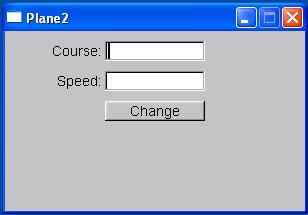
\includegraphics[width=0.50\textwidth]{images/plane.jpg}
	\caption{GUI of Plane}
	\label{fig:plane}
\end{figure}
		
		
	\item \verb SimulationServer:  This  component should be instantiated once in a simulation scenario. It retrieves the position of all planes in a synchronous manner. Radar station can get information about the planes that are in their area of observation. The simulation server computes this based on the location position provided by the radar stations. This component does not expose a graphical user interface.
	
	\item \verb Radar:  This component simulates a radar station. The component acquire the information about the planes that are currently in its area of observation by sending a synchronous request to the simulation server. In this request the radar station provide its own location. The information about the planes is then  presented to the user in a graphical form. Furthermore, the radar station provides the information about the planes in the area of observation to the \verb TAPDisplay  in a asynchronous manner.

\begin{figure}[htbp]
	\centering
		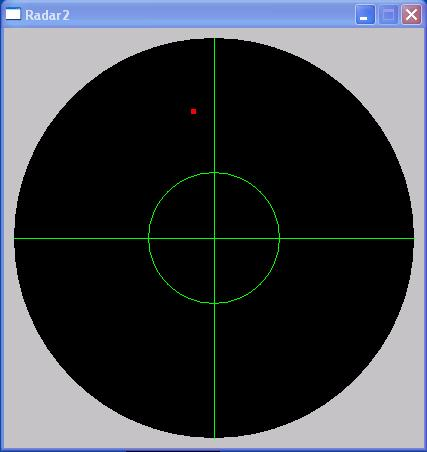
\includegraphics[width=0.50\textwidth]{images/radar.jpg}
	\caption{GUI of Radar station}
	\label{fig:radar}
\end{figure}


\item \verb TAPDisplay:  This component gets information from all radar station about the position of the radar station and the planes in the area of observation. The \verb TAPDisplay  presents the information gathered from all radar stations to the user in a single view.

\begin{figure}[htbp]
	\centering
		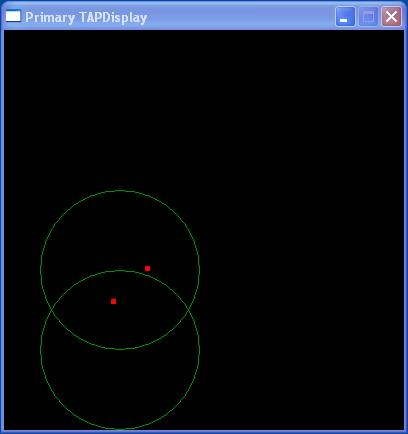
\includegraphics[width=0.50\textwidth]{images/TAPDisplay.jpg}
	\caption{GUI of TAPDisplay}
	\label{fig:TAPDisplay}
\end{figure}
 	
\end{itemize}



\end{document}

